\documentclass[tikz]{standalone}
\usepackage{fourier}
\usepackage{tikz}

\begin{document}
  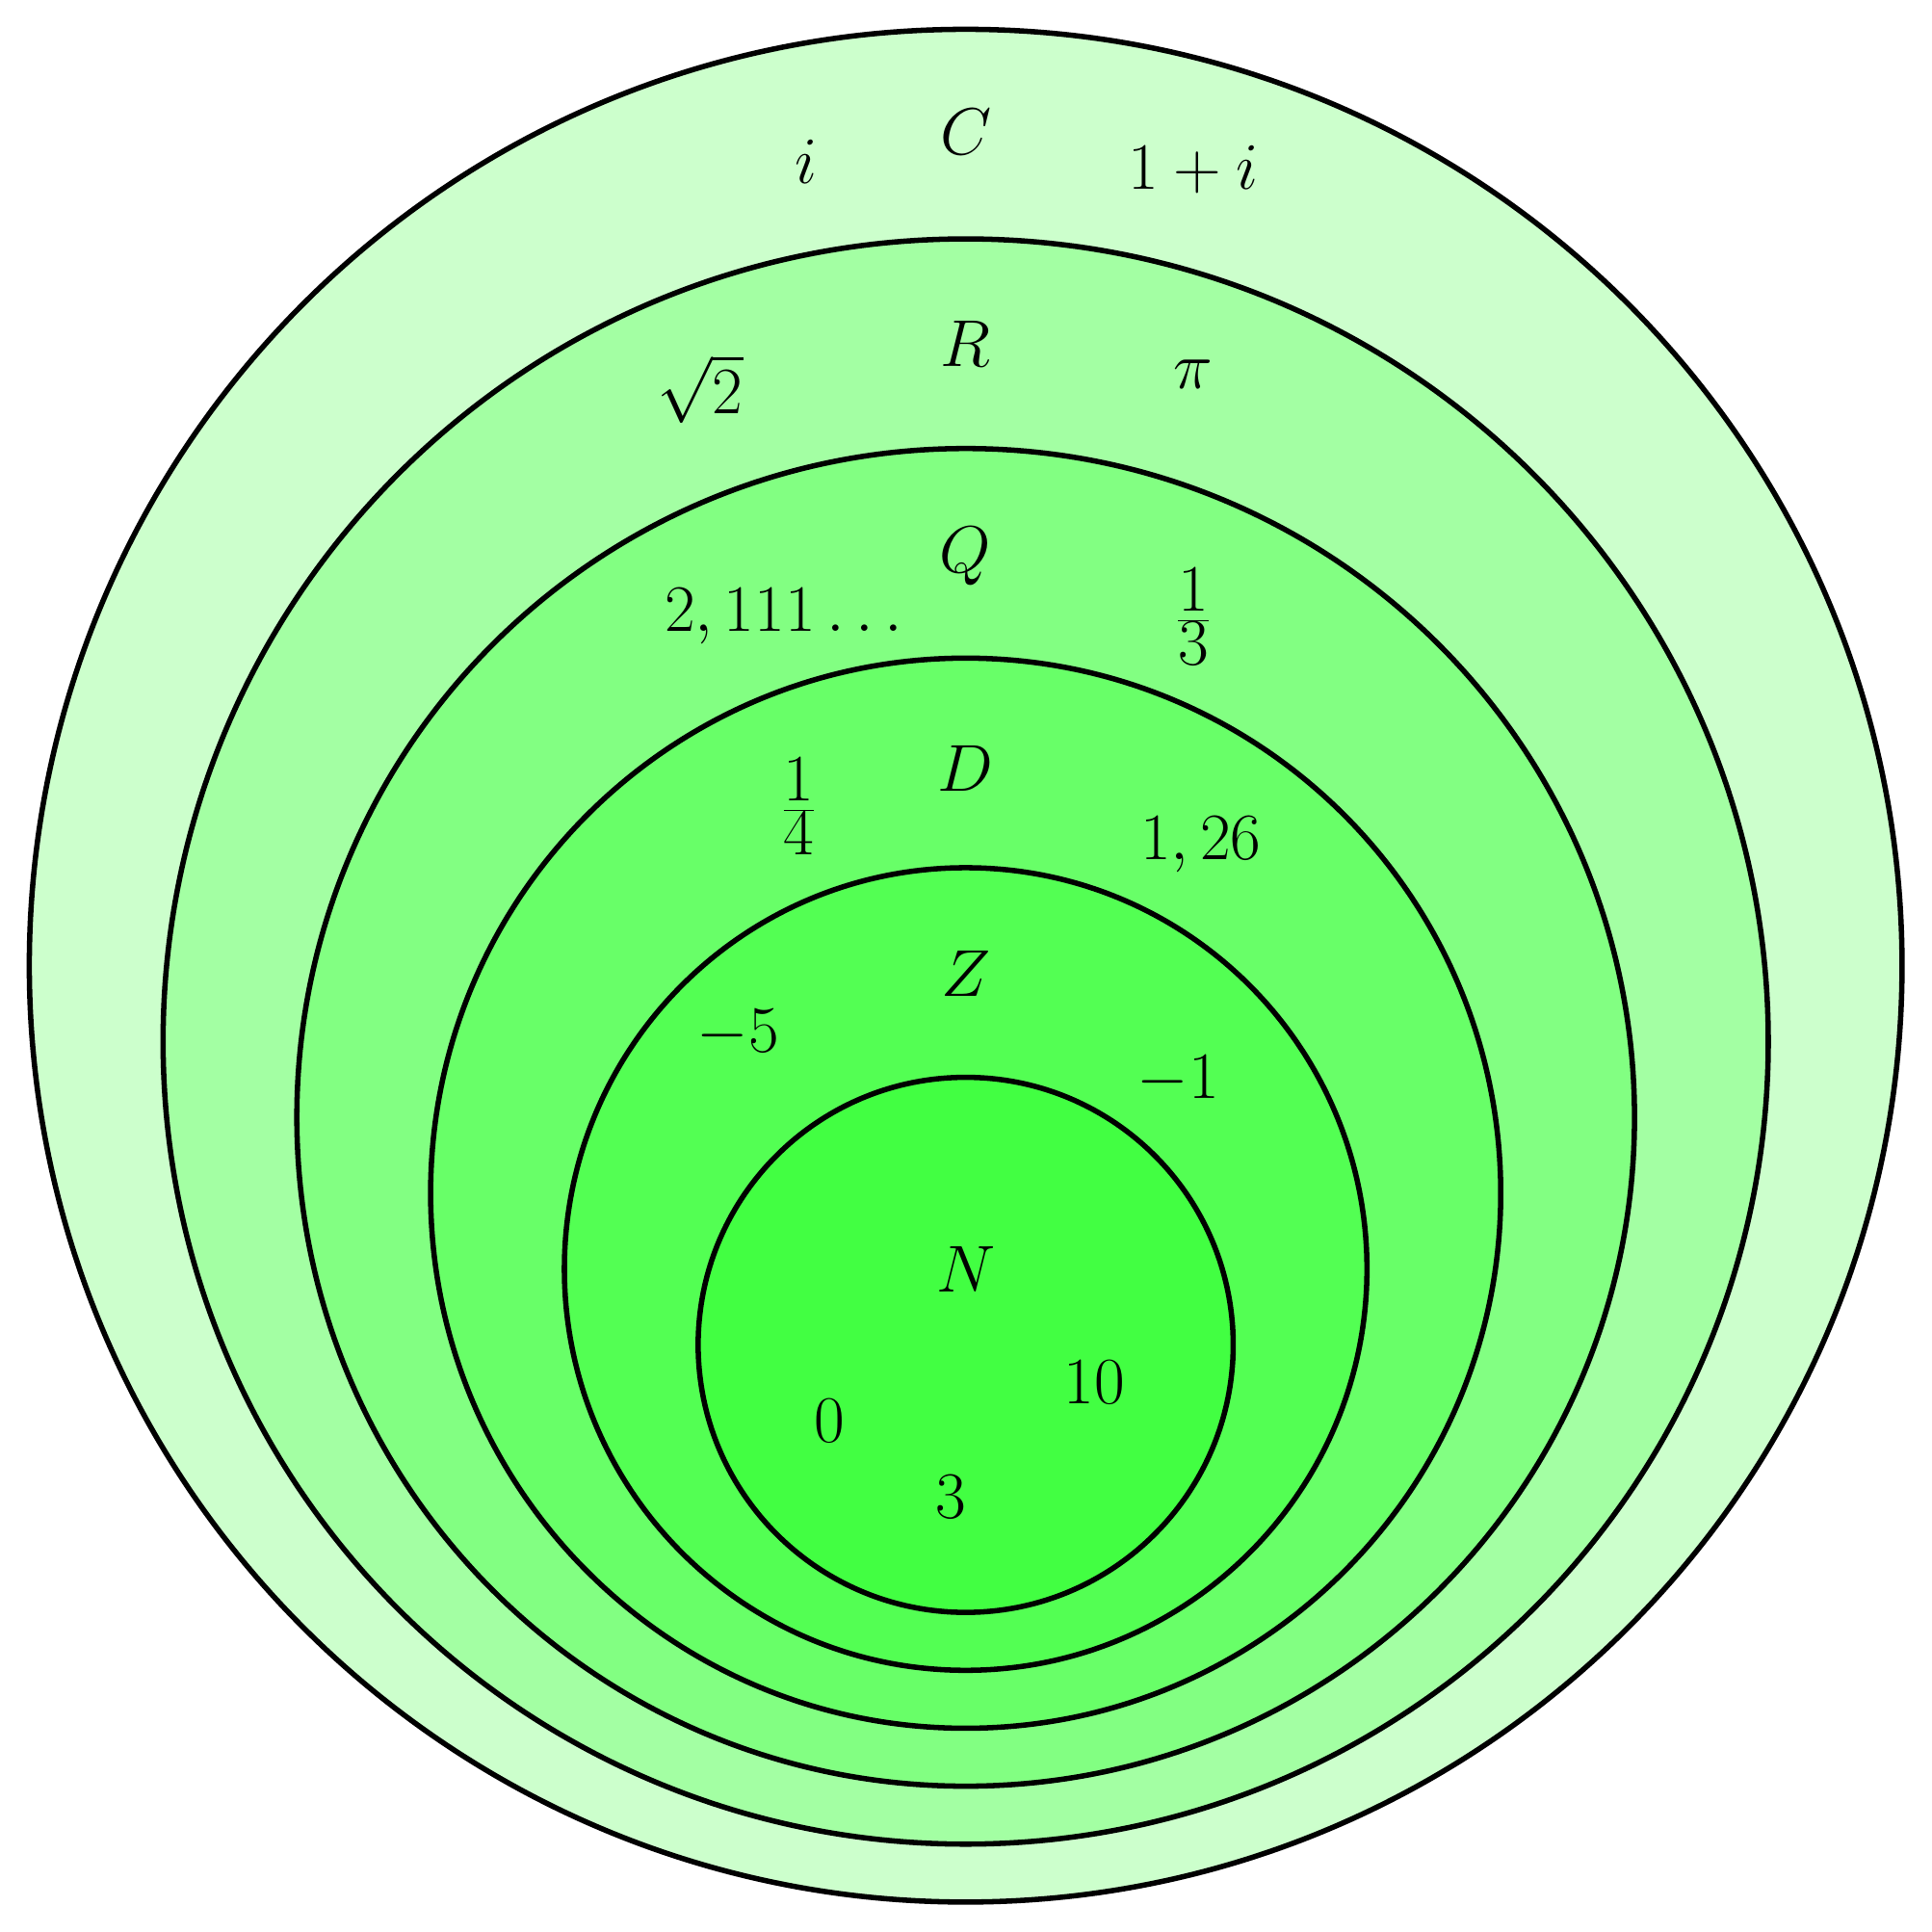
\begin{tikzpicture}
    \draw[black, line width=2pt, fill=green, fill opacity=0.2] (0,0) circle (350px);
    \draw[black, line width=2pt, fill=green, fill opacity=0.2] (0,-1) circle (300px);
    \draw[black, line width=2pt, fill=green, fill opacity=0.2] (0,-2) circle (250px);
    \draw[black, line width=2pt, fill=green, fill opacity=0.2] (0,-3) circle (200px);
    \draw[black, line width=2pt, fill=green, fill opacity=0.2] (0,-4) circle (150px);
    \draw[black, line width=2pt, fill=green, fill opacity=0.2] (0,-5) circle (100px);
    \draw(0,-4) node {\fontsize{70}{80}\selectfont $\mathbb{N}$};
    \draw(-1.8,-6) node {\fontsize{40}{50}\selectfont $0$};
    \draw(-0.2,-7) node {\fontsize{40}{50}\selectfont $3$};
    \draw(1.7,-5.5) node {\fontsize{40}{50}\selectfont $10$};
    \draw(0,-0.1) node {\fontsize{70}{80}\selectfont $\mathbb{Z}$};
    \draw(-3,-0.9) node {\fontsize{40}{50}\selectfont $-5$};
    \draw(2.8,-1.5) node {\fontsize{40}{50}\selectfont $-1$};
    \draw(0,2.6) node {\fontsize{70}{80}\selectfont $\mathbb{D}$};
    \draw(-2.2,2.1) node {\fontsize{40}{50}\selectfont $\frac{1}{4}$};
    \draw(3.1,1.6) node {\fontsize{40}{50}\selectfont $1,26$};
    \draw(0,5.4) node {\fontsize{70}{80}\selectfont $\mathbb{Q}$};
    \draw(-2.4,4.6) node {\fontsize{40}{50}\selectfont $2,111\dots$};
    \draw(3,4.6) node {\fontsize{40}{50}\selectfont $\frac{1}{3}$};
    \draw(0,8.2) node {\fontsize{70}{80}\selectfont $\mathbb{R}$};
    \draw(-3.5,7.6) node {\fontsize{40}{50}\selectfont $\sqrt{2}$};
    \draw(3,7.8) node {\fontsize{40}{50}\selectfont $\pi$};
    \draw(0,11) node {\fontsize{70}{80}\selectfont $\mathbb{C}$};
    \draw(-2.1,10.6) node {\fontsize{40}{50}\selectfont $i$};
    \draw(3,10.5) node {\fontsize{40}{50}\selectfont $1+i$};
  \end{tikzpicture}
\end{document}
